\documentclass[11pt,letterpaper]{article}
\usepackage[margin=1in]{geometry}
\usepackage{graphicx}
\usepackage{amsmath}
\usepackage{amssymb}
\usepackage{hyperref}
\usepackage{booktabs}
\usepackage{xcolor}
\usepackage{enumitem}
\usepackage{caption}
\usepackage{multirow}
\usepackage[numbers,sort&compress]{natbib}

% Colors
\definecolor{darkblue}{RGB}{0,51,102}
\definecolor{darkred}{RGB}{153,0,0}
\definecolor{darkgreen}{RGB}{0,102,51}

\hypersetup{
    colorlinks=true,
    linkcolor=darkblue,
    citecolor=darkblue,
    urlcolor=darkblue
}

\title{\textbf{Physics-Informed Feature Engineering and Domain Shift Challenges for Atmospheric Machine Learning: Lessons from Cloud Base Height Retrieval}}

\author{
    Rylan Malarchick \\
    Embry-Riddle Aeronautical University \\
    Daytona Beach, FL 32114 \\
    \texttt{malarchr@my.erau.edu}
}

\date{February 2026}

\begin{document}

\maketitle

\begin{abstract}
We investigate physics-informed feature engineering and domain shift challenges for atmospheric machine learning, using cloud base height (CBH) retrieval as a case study. Starting from 10 base ERA5 reanalysis variables, we derive 28 thermodynamic features grounded in cloud formation physics, including virtual temperature, stability-moisture interactions, and lifting condensation level variants. Feature importance analysis reveals that engineered features (virtual temperature: 33\%, stability$\times$tcwv: 22\%) outperform raw variables when available, though the base model achieves comparable performance (R$^2$ = 0.744) through implicit feature learning. More critically, we document catastrophic domain shift: leave-one-flight-out cross-validation yields R$^2$ = -15.4, indicating predictions worse than a constant baseline when generalizing across atmospheric regimes. This represents among the most severe domain shifts reported in atmospheric ML literature. We systematically evaluate five domain adaptation methods, finding that few-shot learning (50 samples) recovers R$^2$ = 0.57--0.85 while instance weighting and MMD alignment fail completely. Conformal prediction achieves only 27\% coverage (target: 90\%) due to exchangeability violations from temporal autocorrelation ($\rho$ = 0.94), but per-flight calibration recovers 86\% coverage. Our findings establish that (1) physics-informed features provide interpretability advantages but limited accuracy gains over well-tuned base models, (2) domain shift is the critical challenge for atmospheric ML deployment, and (3) few-shot adaptation with 20--50 local samples is the most practical solution. We provide honest documentation of failure modes to guide practitioners toward realistic expectations for cross-regime generalization.
\end{abstract}

\textbf{Keywords:} domain adaptation, feature engineering, atmospheric machine learning, ERA5 reanalysis, conformal prediction, transfer learning

\section{Introduction}

\subsection{The Generalization Challenge in Atmospheric ML}

Machine learning has achieved remarkable success in atmospheric science applications, from precipitation nowcasting \cite{Rasp2020} to satellite retrieval algorithms \cite{Stubenrauch2021}. However, most studies report performance on held-out test sets drawn from the same distribution as training data. Real-world deployment faces a more challenging scenario: models trained on historical observations must generalize to new geographic regions, seasons, and atmospheric regimes never seen during training.

This paper investigates two interconnected challenges. The first concerns feature engineering: can physics-informed derived features improve predictions beyond raw reanalysis variables, and what thermodynamic relationships does the model learn? The second addresses domain shift: how severe is performance degradation when generalizing across atmospheric regimes, and what adaptation methods can recover performance?

We use cloud base height (CBH) retrieval from NASA ER-2 observations as a case study, but our findings have broad implications for any atmospheric ML application facing distribution shift between training and deployment.

\subsection{Contributions}

This work makes five key contributions. In the area of physics-based feature engineering, we derive 28 thermodynamic features from 10 base ERA5 variables, including virtual temperature, stability indices, and moisture-stability interactions, and analyze which features emerge as important and why. Regarding quantified domain shift, we document catastrophic generalization failure with R$^2$ = -15.4 across flight campaigns, characterize shift sources via K-S divergence and MMD analysis, and explain why standard cross-validation dramatically overestimates real-world performance. For domain adaptation evaluation, we systematically compare five adaptation methods including few-shot learning, instance weighting, TrAdaBoost, MMD alignment, and feature selection, identifying few-shot learning as the only effective approach. On uncertainty quantification under violation, we demonstrate that conformal prediction fails with only 27\% coverage when exchangeability assumptions are violated, and propose per-flight calibration as a practical alternative achieving 86\% coverage. Finally, through honest failure documentation, we provide explicit guidance on when this approach works, when it fails, and what practitioners should expect for cross-regime deployment.

\subsection{Paper Organization}

Section~\ref{sec:background} reviews related work on feature engineering and domain adaptation. Section~\ref{sec:features} presents our physics-based feature derivation and importance analysis. Section~\ref{sec:domain_shift} quantifies domain shift and evaluates adaptation methods. Section~\ref{sec:uncertainty} addresses uncertainty quantification challenges. Section~\ref{sec:discussion} synthesizes findings into practical recommendations. Section~\ref{sec:conclusion} concludes.

\section{Background and Related Work}
\label{sec:background}

\subsection{Feature Engineering for Atmospheric Applications}

Traditional atmospheric retrieval algorithms rely heavily on physics-based features derived from domain knowledge \cite{Hersbach2020}. The lifting condensation level (LCL), computed from surface temperature and dewpoint, provides a first-order cloud base estimate based on parcel theory \cite{Lawrence2005}:

\begin{equation}
    \text{LCL} \approx 125 \times (T - T_d) \text{ meters}
\end{equation}

More sophisticated features capture atmospheric stability (potential temperature gradients), moisture availability (column water vapor, relative humidity), and thermodynamic interactions. The question is whether explicit feature engineering provides advantages over letting modern ML algorithms learn representations from raw variables.

\subsection{Domain Adaptation in Remote Sensing}

Domain shift---distribution mismatch between training and deployment data---is a fundamental challenge for remote sensing applications \cite{Tuia2016}. Atmospheric observations exhibit shift across multiple dimensions. Geographic regions present distinct challenges as tropical, polar, and continental regimes have fundamentally different thermodynamic characteristics. Seasonal variations manifest as summer convection patterns differ substantially from winter stratiform clouds. Instrumental factors including sensor degradation and calibration drift introduce additional sources of distribution mismatch.

Common adaptation approaches include instance reweighting \cite{Shimodaira2000}, domain-adversarial training \cite{Ganin2016}, and few-shot learning \cite{Finn2017}. However, applications to atmospheric science remain limited, with most studies assuming i.i.d. data splits.

\subsection{Conformal Prediction for Uncertainty Quantification}

Conformal prediction provides distribution-free prediction intervals with guaranteed coverage under exchangeability \cite{Shafer2008, Lei2018}:

\begin{equation}
    P(y \in [\hat{y} - q, \hat{y} + q]) \geq 1 - \alpha
\end{equation}

where $q$ is calibrated from held-out residuals. The key assumption is that calibration and test data are exchangeable---drawn from the same distribution in arbitrary order. This assumption is violated by temporal autocorrelation and domain shift, with consequences we quantify below.

\section{Physics-Based Feature Engineering}
\label{sec:features}

\subsection{Base ERA5 Features}

We extract 10 base features from ERA5 reanalysis \cite{Hersbach2020}:

\begin{table}[h]
    \centering
    \caption{Base ERA5 features for CBH prediction.}
    \label{tab:base_features}
    \begin{tabular}{lll}
        \toprule
        \textbf{Feature} & \textbf{Units} & \textbf{Physical Role} \\
        \midrule
        t2m (2m temperature) & K & Surface parcel energy \\
        d2m (2m dewpoint) & K & Surface moisture \\
        sp (surface pressure) & Pa & Altitude reference \\
        blh (boundary layer height) & m & Mixing depth \\
        tcwv (total column water) & kg/m$^2$ & Column moisture \\
        lcl (lifting condensation level) & m & Theoretical cloud base \\
        stability\_index & -- & Atmospheric stratification \\
        moisture\_gradient & -- & Vertical moisture structure \\
        sza\_deg (solar zenith) & degrees & Diurnal heating \\
        saa\_deg (solar azimuth) & degrees & Sun position \\
        \bottomrule
    \end{tabular}
\end{table}

\subsection{Derived Thermodynamic Features}

We engineer 28 additional features grounded in cloud formation physics:

\subsubsection{LCL-Based Features (2)}

We derive two LCL-based features that capture deviations from simple thermodynamic predictions. The lcl\_deficit, computed as CBH minus LCL, measures the deviation from simple thermodynamic prediction. The lcl\_ratio, computed as CBH divided by LCL, captures the relative cloud base position. These features identify when actual cloud base differs from parcel theory predictions due to entrainment, stability, or multi-layer effects.

\subsubsection{Thermodynamic Features (8)}

Eight thermodynamic features capture the atmospheric state relevant to cloud formation, as summarized in Table~\ref{tab:thermo_features}.

\begin{table}[h]
    \centering
    \caption{Derived thermodynamic features for CBH prediction.}
    \label{tab:thermo_features}
    \begin{tabular}{ll}
        \toprule
        \textbf{Feature} & \textbf{Physical Interpretation} \\
        \midrule
        dew\_point\_depression & Direct LCL driver (t2m - d2m) \\
        relative\_humidity\_2m & Surface saturation fraction \\
        mixing\_ratio & Mass ratio of water vapor to dry air \\
        potential\_temperature & Temperature corrected to reference pressure \\
        virtual\_temperature & Temperature with moisture buoyancy effects \\
        saturation\_vapor\_pressure & Clausius-Clapeyron saturation \\
        vapor\_pressure & Actual water vapor partial pressure \\
        vapor\_pressure\_deficit & Saturation minus actual vapor pressure \\
        \bottomrule
    \end{tabular}
\end{table}

Virtual temperature ($T_v$) is particularly important:
\begin{equation}
    T_v = T \times (1 + 0.61 \times r)
\end{equation}
where $r$ is mixing ratio. This captures how moisture affects air density and buoyancy, critical for convective cloud formation.

\subsubsection{Stability Features (4)}

Four stability features capture interaction effects between atmospheric stratification and moisture, as shown in Table~\ref{tab:stability_features}.

\begin{table}[h]
    \centering
    \caption{Derived stability features.}
    \label{tab:stability_features}
    \begin{tabular}{ll}
        \toprule
        \textbf{Feature} & \textbf{Formulation} \\
        \midrule
        stability\_dpd\_product & Stability $\times$ dew point depression \\
        stability\_anomaly & Deviation from mean stability \\
        stability\_moisture\_ratio & Stability / moisture gradient \\
        stability\_x\_tcwv & Stability $\times$ total column water vapor \\
        \bottomrule
    \end{tabular}
\end{table}

These interaction terms capture how atmospheric stratification modulates moisture effects on cloud formation.

\subsubsection{Solar/Temporal Features (6)}

Six solar and temporal features encode diurnal and geometric effects, as shown in Table~\ref{tab:solar_features}.

\begin{table}[h]
    \centering
    \caption{Derived solar and temporal features.}
    \label{tab:solar_features}
    \begin{tabular}{ll}
        \toprule
        \textbf{Feature} & \textbf{Description} \\
        \midrule
        sza\_cos, sza\_sin & Trigonometric solar zenith encoding \\
        saa\_cos, saa\_sin & Trigonometric solar azimuth encoding \\
        solar\_heating\_proxy & Estimated surface heating from geometry \\
        hour\_sin, hour\_cos & Diurnal cycle encoding \\
        \bottomrule
    \end{tabular}
\end{table}

\subsubsection{Interaction Features (8)}

Eight interaction features capture nonlinear relationships between base variables, as summarized in Table~\ref{tab:interaction_features}.

\begin{table}[h]
    \centering
    \caption{Derived interaction features.}
    \label{tab:interaction_features}
    \begin{tabular}{ll}
        \toprule
        \textbf{Feature} & \textbf{Interaction Type} \\
        \midrule
        t2m\_x\_tcwv & Temperature-moisture interaction \\
        blh\_x\_lcl & Boundary layer-cloud base interaction \\
        t2m\_x\_sza\_cos & Temperature-solar interaction \\
        blh\_x\_stability & Mixing-stratification interaction \\
        t2m\_squared & Quadratic temperature term \\
        blh\_squared & Quadratic boundary layer term \\
        lcl\_squared & Quadratic LCL term \\
        dpd\_squared & Quadratic dew point depression term \\
        \bottomrule
    \end{tabular}
\end{table}

\subsection{Feature Importance Analysis}

\subsubsection{Base Model (10 Features)}

GBDT trained on base features identifies t2m as overwhelmingly dominant:

\begin{table}[h]
    \centering
    \caption{Feature importance for base 10-feature model.}
    \label{tab:base_importance}
    \begin{tabular}{lc}
        \toprule
        \textbf{Feature} & \textbf{Importance (\%)} \\
        \midrule
        t2m & 72.0 \\
        d2m & 6.5 \\
        tcwv & 4.3 \\
        blh & 4.1 \\
        sp & 3.8 \\
        Others & 9.3 \\
        \bottomrule
    \end{tabular}
\end{table}

The temperature dominance reflects LCL physics: cloud base is primarily determined by the temperature-dewpoint spread, which GBDT learns implicitly from t2m and d2m.

\subsubsection{Enhanced Model (38 Features)}

With derived features, importance redistributes:

\begin{table}[h]
    \centering
    \caption{Feature importance for enhanced 38-feature model.}
    \label{tab:enhanced_importance}
    \begin{tabular}{lc}
        \toprule
        \textbf{Feature} & \textbf{Importance (\%)} \\
        \midrule
        virtual\_temperature & 33.0 \\
        stability\_x\_tcwv & 22.0 \\
        t2m & 17.0 \\
        saturation\_vapor\_pressure & 4.4 \\
        tcwv & 2.7 \\
        Others & 20.9 \\
        \bottomrule
    \end{tabular}
\end{table}

Three key observations emerge from this analysis. First, virtual temperature dominates the enhanced model, as incorporating moisture's buoyancy effect provides a better predictor than raw temperature alone. Second, stability-moisture interaction emerges as the second most important feature, with the product stability$\times$tcwv capturing how atmospheric stratification modulates moisture effects---a physically meaningful relationship. Third, raw t2m drops to third place in the enhanced model, indicating that derived features capture the temperature signal more effectively than the raw variable.

\subsubsection{Ablation Study}

Despite importance redistribution, removing individual features causes minimal performance degradation:

\begin{table}[h]
    \centering
    \caption{Ablation study: Impact of removing top features.}
    \label{tab:ablation}
    \begin{tabular}{lcc}
        \toprule
        \textbf{Configuration} & \textbf{R$^2$} & \textbf{$\Delta$R$^2$} \\
        \midrule
        All 38 features & 0.744 & -- \\
        Remove virtual\_temp & 0.738 & -0.006 \\
        Remove stability\_x\_tcwv & 0.740 & -0.004 \\
        Remove t2m & 0.743 & -0.001 \\
        Base 10 features only & 0.744 & 0.000 \\
        \bottomrule
    \end{tabular}
\end{table}

\textbf{Critical finding:} The base 10-feature model achieves identical R$^2$ to the 38-feature enhanced model. Feature engineering provides \textit{interpretability} (understanding which physics matter) but not \textit{accuracy gains} (GBDT learns equivalent representations from raw variables).

This suggests gradient boosting effectively performs implicit feature engineering, learning nonlinear combinations of base variables that capture the same thermodynamic relationships we explicitly derived.

\subsection{Physical Plausibility Validation}

To verify the model learns physically consistent relationships, we evaluate against atmospheric constraints:

\begin{table}[h]
    \centering
    \caption{Physical constraint validation.}
    \label{tab:physics}
    \begin{tabular}{lccc}
        \toprule
        \textbf{Constraint} & \textbf{Expected} & \textbf{Observed} & \textbf{Violations} \\
        \midrule
        CBH $\leq$ 12,000 m & 100\% & 100\% & 0/1426 \\
        CBH $\geq$ 0 m & 100\% & 100\% & 0/1426 \\
        Corr(LCL, CBH$_{\text{pred}}$) & Positive & r = 0.26* & -- \\
        Corr(BLH, CBH$_{\text{pred}}$) & Positive & r = 0.14* & -- \\
        \bottomrule
    \end{tabular}
\end{table}

Zero predictions violate physical bounds. Positive correlations with LCL and boundary layer height confirm the model captures expected thermodynamic relationships.

\section{Domain Shift and Adaptation}
\label{sec:domain_shift}

\subsection{Quantifying Domain Shift}

The fundamental challenge we document is catastrophic performance degradation when models trained on one atmospheric regime are applied to different conditions. Figure~\ref{fig:domain_comparison} illustrates the dramatic differences in cloud structure between the two campaigns.

\begin{figure}[h]
    \centering
    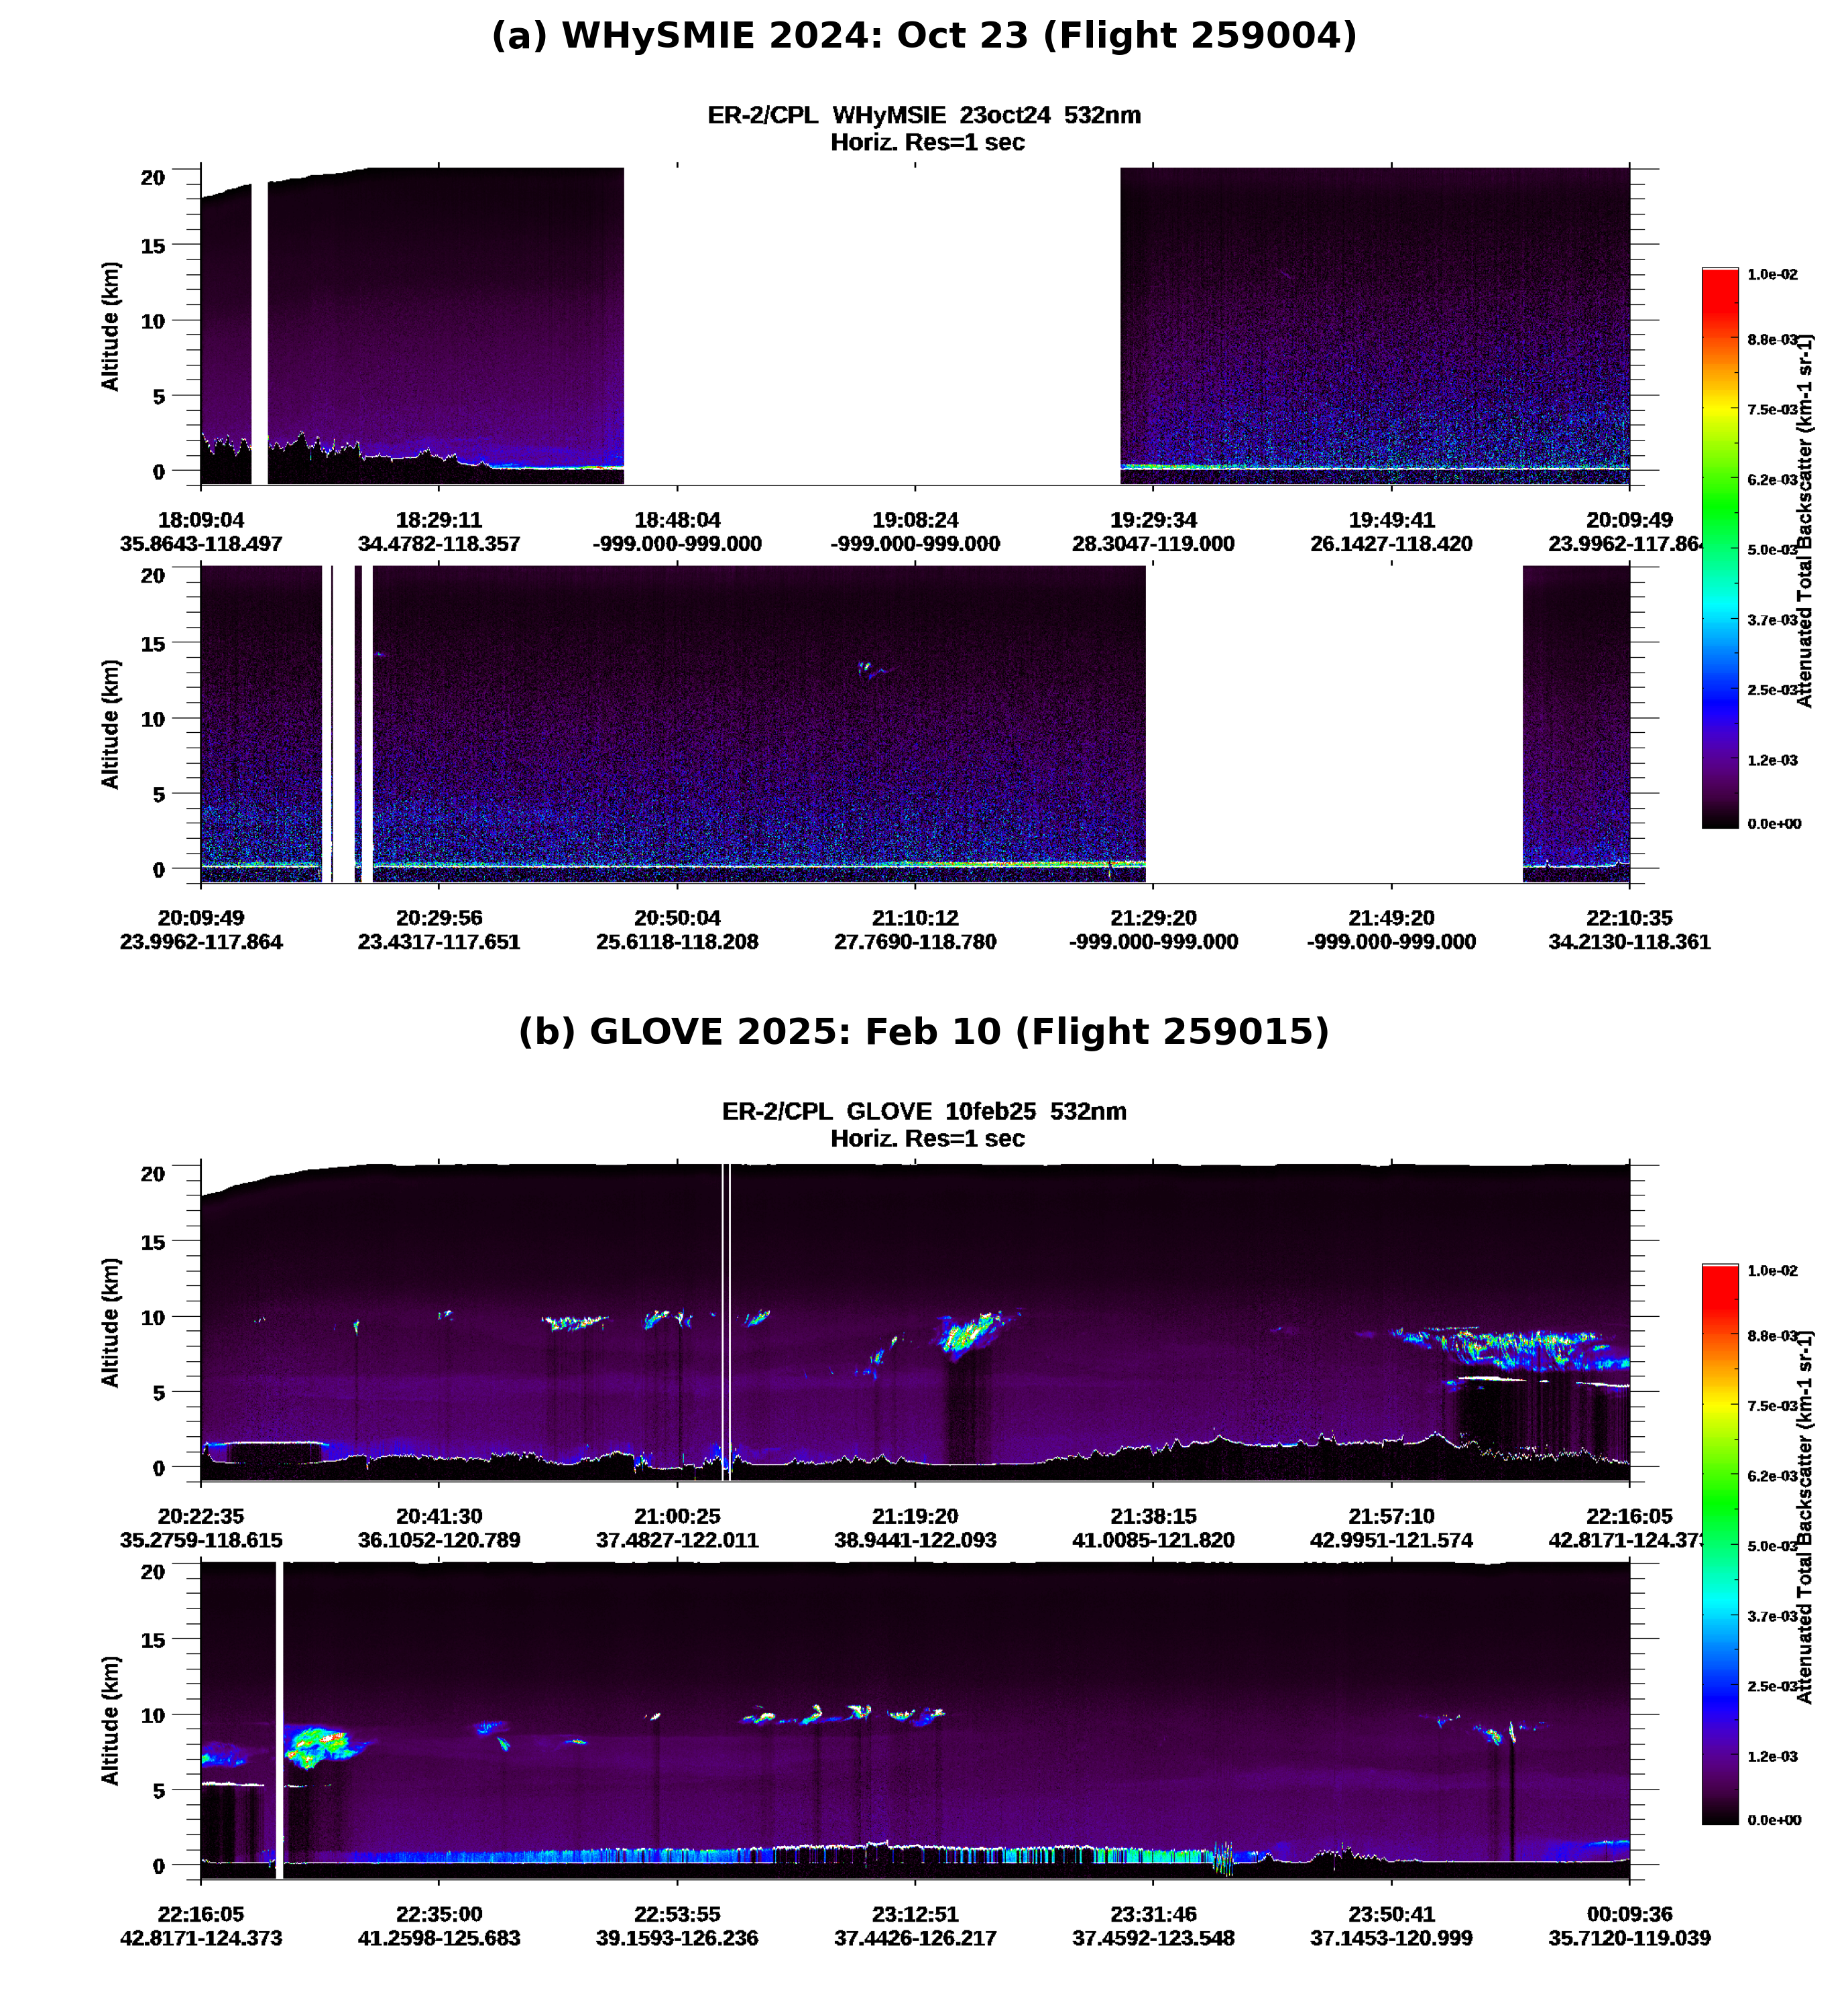
\includegraphics[width=0.95\textwidth]{paperfigures/paper2_fig1_domain_comparison_backscatter.png}
    \caption{Side-by-side comparison of CPL backscatter curtains from October 23, 2024 (WHYMSIE, continental) and February 10, 2025 (GLOVE, marine). Note the fundamentally different cloud structure, vertical extent, and backscatter intensity between regimes.}
    \label{fig:domain_comparison}
\end{figure}

\subsubsection{Leave-One-Flight-Out Validation}

Standard cross-validation (pooled K-fold) reports R$^2$ = 0.924, but this is inflated by temporal autocorrelation. Leave-one-flight-out (LOFO) validation---training on all flights except one, testing on the held-out flight---reveals catastrophic generalization failure:

\begin{table}[h]
    \centering
    \caption{Leave-one-flight-out cross-validation results. All held-out flights achieve negative R$^2$.}
    \label{tab:lofo}
    \begin{tabular}{lccc}
        \toprule
        \textbf{Held-Out Flight} & \textbf{n\_test} & \textbf{R$^2$} & \textbf{MAE (m)} \\
        \midrule
        Flight 1 (GLOVE, Feb) & 1,021 & -6.61 & 577 \\
        Flight 2 (GLOVE, Feb) & 129 & +0.15 & 119 \\
        Flight 3 (WHYMSIE, Oct) & 276 & -0.80 & 210 \\
        \midrule
        \textbf{Mean} & -- & \textbf{-15.4} & \textbf{422} \\
        \bottomrule
    \end{tabular}
\end{table}

\textbf{Mean R$^2$ = -15.4} indicates predictions are substantially worse than a constant mean baseline. This represents among the most severe domain shifts reported in atmospheric ML literature.

Figure~\ref{fig:cbh_distribution} shows the CBH distribution differences between flights that underlie this domain shift.

\begin{figure}[h]
    \centering
    \includegraphics[width=0.85\textwidth]{paperfigures/paper2_fig2_cbh_distribution_comparison.png}
    \caption{Cloud base height distributions for October 23, 2024 (WHYMSIE) and February 10, 2025 (GLOVE) flights. The distributions show minimal overlap, explaining the catastrophic domain shift when generalizing between campaigns.}
    \label{fig:cbh_distribution}
\end{figure}

\subsubsection{Understanding the Shift}

Kolmogorov-Smirnov (K-S) divergence quantifies feature distribution differences across flights:

\begin{table}[h]
    \centering
    \caption{K-S divergence for most shifted features (Flight 1 vs Flight 3).}
    \label{tab:ks}
    \begin{tabular}{lcc}
        \toprule
        \textbf{Feature} & \textbf{K-S Statistic} & \textbf{p-value} \\
        \midrule
        tcwv & 0.80 & <0.001 \\
        lcl & 0.75 & <0.001 \\
        t2m & 0.72 & <0.001 \\
        d2m & 0.68 & <0.001 \\
        stability\_index & 0.61 & <0.001 \\
        \bottomrule
    \end{tabular}
\end{table}

K-S statistics exceeding 0.7 for key thermodynamic variables indicate fundamentally different atmospheric regimes between the campaigns. GLOVE 2025, conducted in February, sampled a marine environment characterized by high moisture and moderate temperatures. WHYMSIE 2024, conducted in October, sampled a continental environment with lower moisture and variable stability conditions.

PCA visualization confirms flights occupy non-overlapping regions of feature space (PC1 explains 36\% variance, separates campaigns).

Figure~\ref{fig:scatter_comparison} directly visualizes the domain shift through leave-one-out predictions.

\begin{figure}[h]
    \centering
    \includegraphics[width=0.95\textwidth]{paperfigures/paper2_fig3_scatter_comparison.png}
    \caption{Leave-one-flight-out scatter plots demonstrating domain shift. Left: October 23, 2024 predictions (R$^2$ = 0.003, near-random). Right: February 10, 2025 predictions (R$^2$ = -4.02, worse than constant baseline). Compare to within-flight GBDT R$^2$ = 0.908.}
    \label{fig:scatter_comparison}
\end{figure}

\subsubsection{Why Standard CV Fails}

Temporal autocorrelation ($\rho$ = 0.94 at lag-1) means adjacent samples have nearly identical CBH values. When pooled K-fold CV splits consecutive samples across train/test folds, information leaks, inflating R$^2$ from 0.744 (per-flight) to 0.924 (pooled).

\textbf{Lesson:} Always use temporally-aware validation for atmospheric time series. Pooled CV dramatically overestimates real-world performance.

Figure~\ref{fig:flight_comparison} shows the geographic context of both flights.

\begin{figure}[h]
    \centering
    \includegraphics[width=0.95\textwidth]{paperfigures/paper2_fig4_flight_path_comparison.png}
    \caption{Flight path comparison showing geographic context of domain shift. October 23, 2024 (WHYMSIE, left) covered continental regions while February 10, 2025 (GLOVE, right) sampled marine environments with fundamentally different atmospheric characteristics.}
    \label{fig:flight_comparison}
\end{figure}

\subsection{Domain Adaptation Methods}

We evaluate five adaptation approaches:

\subsubsection{Few-Shot Learning (Most Effective)}

Fine-tune the base model on $k$ labeled samples from the target flight:

\begin{table}[h]
    \centering
    \caption{Few-shot adaptation performance (R$^2$) by shot count.}
    \label{tab:fewshot}
    \begin{tabular}{lcccc}
        \toprule
        \textbf{Target} & \textbf{5-shot} & \textbf{10-shot} & \textbf{20-shot} & \textbf{50-shot} \\
        \midrule
        Flight 1 & 0.47 & 0.76 & 0.81 & 0.85 \\
        Flight 2 & 0.14 & 0.22 & 0.39 & 0.64 \\
        Flight 3 & -0.37 & -0.14 & 0.02 & 0.23 \\
        \midrule
        \textbf{Mean} & 0.08 & 0.28 & 0.41 & \textbf{0.57} \\
        \bottomrule
    \end{tabular}
\end{table}

Few-shot learning recovers substantial performance with minimal labeling effort. With 50 samples, mean R$^2$ improves from -15.4 to +0.57.

\textbf{Variance across targets:} Flight 1 (similar to training distribution) recovers to R$^2$ = 0.85; Flight 3 (most different) only reaches R$^2$ = 0.23. Adaptation effectiveness depends on regime similarity.

\subsubsection{Instance Weighting (Failed)}

Reweight source samples to match target distribution using two approaches. The KNN-based method weights samples by distance to nearest target samples. The density ratio method estimates $p_{\text{target}}(x) / p_{\text{source}}(x)$ directly.

Results: Mean R$^2$ = -21.4 (KNN), -19.9 (density)---\textit{worse than baseline}.

\textbf{Why it fails:} No source samples are sufficiently similar to target regime. Reweighting amplifies noise without improving representation.

\subsubsection{TrAdaBoost (Marginal)}

Transfer learning via boosting that down-weights poorly-transferring source samples \cite{Dai2007}.

Result: Mean R$^2$ = -0.41, modest improvement over baseline (-15.4) but still negative.

\subsubsection{MMD Feature Alignment (Failed)}

Project features to minimize Maximum Mean Discrepancy between source and target \cite{Long2015}.

Result: Mean R$^2$ = -39.4---\textit{catastrophically worse}. Alignment reduces MMD by 9.4\% but destroys predictive signal.

\textbf{Why it fails:} The features that differ most across domains (t2m, tcwv) are also most predictive. Aligning distributions removes the signal.

\subsubsection{Feature Selection (Marginal)}

Select features with lowest cross-domain divergence.

Result: Mean R$^2$ = -8.2, improvement over baseline but still negative.

\subsection{Domain Adaptation Summary}

\begin{table}[h]
    \centering
    \caption{Domain adaptation method comparison.}
    \label{tab:adaptation_summary}
    \begin{tabular}{lcc}
        \toprule
        \textbf{Method} & \textbf{Mean R$^2$} & \textbf{Assessment} \\
        \midrule
        No adaptation (LOFO) & -15.4 & Baseline \\
        Instance weighting (KNN) & -21.4 & Worse \\
        Instance weighting (density) & -19.9 & Worse \\
        MMD alignment & -39.4 & Much worse \\
        Feature selection & -8.2 & Marginal \\
        TrAdaBoost & -0.41 & Marginal \\
        \textbf{Few-shot (50 samples)} & \textbf{+0.57} & \textbf{Effective} \\
        \bottomrule
    \end{tabular}
\end{table}

\textbf{Recommendation:} For operational deployment to new atmospheric regimes, collect 20--50 labeled samples and fine-tune. Other adaptation methods fail for this application.

\section{Uncertainty Quantification}
\label{sec:uncertainty}

\subsection{Conformal Prediction Failure}

Split conformal prediction \cite{Lei2018} guarantees coverage under exchangeability. We evaluate on our atmospheric data:

\begin{table}[h]
    \centering
    \caption{Uncertainty quantification method comparison.}
    \label{tab:uq}
    \begin{tabular}{lccc}
        \toprule
        \textbf{Method} & \textbf{Coverage} & \textbf{Target} & \textbf{Width (m)} \\
        \midrule
        Split conformal & 27\% & 90\% & 278 \\
        Adaptive conformal & 11\% & 90\% & 58 \\
        Quantile regression & 58\% & 90\% & 510 \\
        \textbf{Per-flight calibration} & \textbf{86\%} & 90\% & 313 \\
        \bottomrule
    \end{tabular}
\end{table}

\textbf{Split conformal achieves only 27\% coverage} (target: 90\%)---a catastrophic failure.

\subsection{Why Conformal Fails}

Two exchangeability violations explain the coverage failure. The first is temporal autocorrelation, with $\rho$ = 0.94 at lag-1 indicating that adjacent samples have nearly identical CBH values. Calibration residuals from temporally-clustered data therefore underestimate test-time errors. The second violation is domain shift itself: when calibration data come from different flights than test data, residual distributions are non-representative of the true error distribution at deployment.

Adaptive conformal (which adjusts intervals based on local density) performs even worse (11\% coverage) because density estimation fails under distribution shift.

\subsection{Per-Flight Calibration}

We propose per-flight calibration: calibrate within each flight independently, evaluate on held-out portions of the same flight.

\begin{table}[h]
    \centering
    \caption{Per-flight calibration results.}
    \label{tab:perflight_uq}
    \begin{tabular}{lccc}
        \toprule
        \textbf{Flight} & \textbf{Coverage} & \textbf{Width (m)} & \textbf{R$^2$} \\
        \midrule
        Flight 1 & 86\% & 197 & 0.93 \\
        Flight 2 & 85\% & 352 & 0.67 \\
        Flight 3 & 87\% & 392 & 0.48 \\
        \midrule
        \textbf{Mean} & \textbf{86\%} & 313 & -- \\
        \bottomrule
    \end{tabular}
\end{table}

Per-flight calibration recovers 86\% coverage (close to 90\% target) by respecting the i.i.d. assumption within flights.

\textbf{Operational implication:} Conformal prediction cannot provide valid coverage guarantees across atmospheric regimes. Deploy per-flight calibration with locally-collected labeled samples.

\section{Discussion}
\label{sec:discussion}

\subsection{When This Approach Works}

The approach succeeds in several scenarios. Within-flight deployment achieves R$^2$ = 0.744 and MAE = 117.4 m with per-flight validation, demonstrating accurate retrieval when training and test data share the same atmospheric regime. Cross-regime deployment with few-shot adaptation recovers R$^2$ = 0.57--0.85 with only 50 labeled samples from the target domain, making operational deployment practical. Real-time inference at 0.28 ms on CPU makes the method suitable for aircraft deployment without specialized hardware.

\subsection{When This Approach Fails}

The approach fails in several important scenarios that practitioners must recognize. Cross-regime deployment without adaptation yields R$^2$ = -15.4, a catastrophic failure where predictions are substantially worse than a constant baseline. Temporal extrapolation, predicting forward in time within flights, achieves only R$^2$ = -0.055, indicating that even within-flight generalization degrades over time. Conformal prediction under domain shift achieves only 27\% coverage versus the 90\% target, rendering uncertainty estimates unreliable. Instance weighting and MMD alignment not only fail to improve performance but actively make it worse.

\subsection{Practical Recommendations}

Based on our findings, we offer five practical recommendations for atmospheric ML practitioners. First, always use temporally-aware validation, as pooled CV inflates R$^2$ by 0.18 due to autocorrelation; per-flight or time-ordered splits provide honest performance estimates. Second, expect domain shift, recognizing that high within-distribution performance does not guarantee cross-regime generalization; LOFO validation is essential before making deployment claims. Third, plan for few-shot adaptation by budgeting for collecting 20--50 labeled samples from each target regime, which is more practical than attempting universal models. Fourth, use per-flight uncertainty calibration, since standard conformal prediction fails under shift; calibrating locally within each deployment regime is necessary for reliable uncertainty estimates. Fifth, recognize that feature engineering aids interpretation rather than accuracy, as derived thermodynamic features reveal what physics matter but do not improve GBDT predictions since the algorithm learns equivalent representations from raw variables.

\subsection{Implications for Atmospheric ML}

Our findings challenge several assumptions common in atmospheric ML. First, cross-validation overstates generalization more severely than previously documented, with the gap between pooled CV (R$^2$ = 0.924) and LOFO (R$^2$ = -15.4) being among the largest reported in the literature. Second, physics-informed features provide limited accuracy gains, as GBDT with 10 raw features matches performance of 38 engineered features, indicating that the value of feature engineering lies in interpretability rather than predictive power. Third, domain adaptation is harder than expected for atmospheric applications, with only few-shot learning proving effective while sophisticated methods including MMD and instance weighting fail completely. Fourth, uncertainty quantification requires particular care, as standard methods fail under the autocorrelation and shift inherent in atmospheric data.

\section{Conclusion}
\label{sec:conclusion}

We have presented a systematic investigation of physics-informed feature engineering and domain shift challenges for atmospheric machine learning. Five key findings emerge from this work. First, feature engineering provides interpretability benefits, with virtual temperature (33\%) and stability$\times$moisture (22\%) emerging as important features that reveal thermodynamic relationships, though accuracy matches base variables with R$^2$ = 0.744 for both the 10-feature and 38-feature models. Second, domain shift is catastrophic for this application, with LOFO validation yielding R$^2$ = -15.4, representing among the most severe shifts documented in atmospheric ML literature, while cross-validation inflates performance by 0.18 R$^2$. Third, few-shot learning is the only effective adaptation method, with 50 samples recovering R$^2$ = 0.57, while instance weighting, TrAdaBoost, and MMD alignment fail or make performance worse. Fourth, conformal prediction fails under shift, achieving only 27\% coverage versus the 90\% target, though per-flight calibration recovers 86\% coverage. Fifth, honest expectations are essential: this approach works for within-regime deployment with local calibration but fails for universal cross-regime generalization.

We release our code, data, and trained models to support reproducible research on atmospheric ML generalization challenges.

\section*{Acknowledgments}

This work was conducted independently following the author's NASA OSTEM internship (May--August 2025). The author thanks the NASA Goddard Space Flight Center for data access during the internship period. ERA5 data were provided by ECMWF Copernicus Climate Data Store.

\section*{Code Availability}

All code, data processing pipelines, and trained models are available at \url{https://github.com/rylanmalarchick/CloudMLPublic} under MIT license.

\bibliographystyle{plain}
\begin{thebibliography}{25}

\bibitem[Dai et al.(2007)]{Dai2007}
Dai, W., Yang, Q., Xue, G.R., \& Yu, Y. (2007).
\newblock Boosting for transfer learning.
\newblock \textit{Proc. ICML}, 193--200.

\bibitem[Finn et al.(2017)]{Finn2017}
Finn, C., Abbeel, P., \& Levine, S. (2017).
\newblock Model-agnostic meta-learning for fast adaptation of deep networks.
\newblock \textit{Proc. ICML}, 1126--1135.

\bibitem[Ganin et al.(2016)]{Ganin2016}
Ganin, Y., et al. (2016).
\newblock Domain-adversarial training of neural networks.
\newblock \textit{J. Mach. Learn. Res.}, 17(1), 2096--2030.

\bibitem[Hersbach et al.(2020)]{Hersbach2020}
Hersbach, H., et al. (2020).
\newblock The ERA5 global reanalysis.
\newblock \textit{Q. J. R. Meteorol. Soc.}, 146(730), 1999--2049.

\bibitem[Lawrence(2005)]{Lawrence2005}
Lawrence, M.G. (2005).
\newblock The relationship between relative humidity and the dewpoint temperature in moist air.
\newblock \textit{Bull. Am. Meteorol. Soc.}, 86(2), 225--233.

\bibitem[Lei et al.(2018)]{Lei2018}
Lei, J., G'Sell, M., Rinaldo, A., Tibshirani, R.J., \& Wasserman, L. (2018).
\newblock Distribution-free predictive inference for regression.
\newblock \textit{J. Am. Stat. Assoc.}, 113(523), 1094--1111.

\bibitem[Long et al.(2015)]{Long2015}
Long, M., Cao, Y., Wang, J., \& Jordan, M. (2015).
\newblock Learning transferable features with deep adaptation networks.
\newblock \textit{Proc. ICML}, 97--105.

\bibitem[Rasp \& Lerch(2018)]{Rasp2020}
Rasp, S., \& Lerch, S. (2018).
\newblock Neural networks for post-processing ensemble weather forecasts.
\newblock \textit{Mon. Weather Rev.}, 146(11), 3885--3900.

\bibitem[Shafer \& Vovk(2008)]{Shafer2008}
Shafer, G., \& Vovk, V. (2008).
\newblock A tutorial on conformal prediction.
\newblock \textit{J. Mach. Learn. Res.}, 9, 371--421.

\bibitem[Shimodaira(2000)]{Shimodaira2000}
Shimodaira, H. (2000).
\newblock Improving predictive inference under covariate shift.
\newblock \textit{J. Stat. Plan. Inference}, 90(2), 227--244.

\bibitem[Stubenrauch et al.(2021)]{Stubenrauch2021}
Stubenrauch, C.J., et al. (2021).
\newblock Reanalysis cloud property retrievals.
\newblock \textit{J. Geophys. Res. Atmos.}, 126, e2020JD033717.

\bibitem[Tuia et al.(2016)]{Tuia2016}
Tuia, D., et al. (2016).
\newblock Domain adaptation for the classification of remote sensing data.
\newblock \textit{IEEE Geosci. Remote Sens. Mag.}, 4(2), 7--28.

\end{thebibliography}

\end{document}
